\section{Einführung}


\subsection{Messen, Steuern, Regeln}

Ziel einer Regelung ist i. Allg., bestimmte Größen, meist Ausgangsgrößen technischer Prozesse, an vorgegebene Führungsgrößen anzugleichen.
Die zu regelnden Größen sollen sowohl Änderungen der Führungsgrößen möglichst gut folgen als auch von Störungen, die auf den Prozess einwirken, möglichst wenig beeinflusst werden.
Die genannten Ziele werden dadurch angestrebt, dass die Regelgrößen gemessen und die Messergebnisse mit den Führungsgrößen verglichen werden.
Aus den Differenzen von Führungs- und Regelgrößen werden Eingriffe in den Prozess abgeleitet, die geeignet sind, die Differenzen zu vermindern.
Durch diese Rückführung von Ausgangsgrößen auf Eingangsgrößen entstehen geschlossene Wirkungsabläufe, die als Regelkreise bezeichnet werden.
Genaue Definitionen von Begriffen und Bezeichnungen in der Regelungs- und Steuerungstechnik finden sich u.a. in der DIN IEC 60050-351 Leittechnik.

Zur Einführung in regelungstechnische Fragestellungen sollen zwei Beispiele betrachtet werden.

Im ersten Beispiel besteht die Aufgabe darin, die Temperatur \(X\) eines Wohnraumes auf einem konstanten, vorgegebenen Wert \(W\) zu halten.
Störungen, wie Änderung der Außentemperatur \(Z_1\), Öffnen und Schließen von Fenstern und Türen \(Z_2\), sollen die Temperatur nicht oder nicht wesentlich beeinflussen.
Die regelungstechnische Lösung besteht darun, dass die Temperatur \(X\) gemessen und das Heizungsventil entsprechend dem Unterschied von gemessenem und vorgegebenem Wert um den Betrag \(Y\) verstellt wird.
Dies kann von Hand oder automatisch durch den Regler \(R\) geschehen.

Bild \ref{fig:1-2} zeigt, wie der durch Bild \ref{fig:1-1} gegebene Sachverhalt un übersichtlicherer und einfacherer Weise dargestellt werden kann.

Dies ist möglich, weil hier nur die wirkungsmäßigen Zusammenhänge interessieren, nicht hingegen die physikalische Realisierung.
Aus dieser schematischen Darstellung ist u.a. zu erkennen, dass die Temperatur \(X\) über Regler und Heizungsvektil sich selbst beeinflusst.
Dieser in sich geschlossene Wirkungsablauf ist ein wichtiges Merkmal jeder Regelung.

\begin{figure}[h]
	\centering
    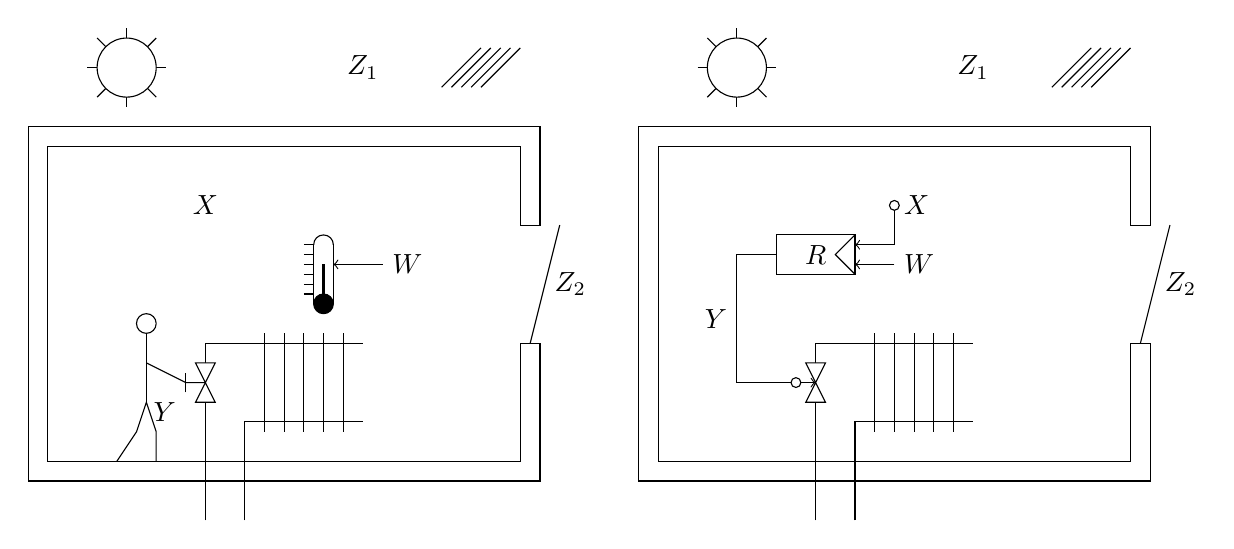
\begin{tikzpicture}
    	\draw (0,0) -- (0,4) -- (6,4) -- (6,3) -- (6.25,3) -- (6.25,4.25) -- (-.25,4.25) -- (-.25,-.25) -- (6.25,-.25) -- (6.25,1.5) -- (6,1.5) -- (6,0) -- cycle; % walls
    	\draw (6.125,1.5) -- (6.5,3) node[midway,right] {\(Z_2\)}; % window
    	% sun
    	\draw (.5,5) -- (1.5,5);
    	\draw (1,5.5) -- (1,4.5);
    	\draw (.625,4.625) -- (1.375,5.375);
    	\draw (.625,5.375) -- (1.375,4.625);
    	\filldraw[fill=white] (1,5) circle (.375);
    	\node at (4,5) {\(Z_1\)};
    	\foreach \i in {0,...,4}
    		\draw (6-.125*\i,5.25) -- (5.5-.125*\i,4.75);
    	 % thermostat
    	\draw (3.5,2.75) circle (.125);
    	\fill[fill=white] (3.375,2) rectangle (3.625,2.75);
    	\draw (3.375,2) -- (3.375,2.75);
    	\draw (3.625,2) -- (3.625,2.75);
    	\filldraw (3.5,2) circle (.125);
    	\draw[thick] (3.5,2) -- (3.5,2.5);
    	\foreach \i in {0,...,5}
    		\draw (3.25,2.125+.125*\i) -- (3.375,2.125+.125*\i);
    	\draw[->] (4.25,2.5) node[right] {\(W\)} -- (3.625,2.5);
    	\node at (2,3.25) {\(X\)};
    	% heater
    	\draw (2,-.75) -- (2,1.5) -- (4,1.5);
    	\draw (2.5,-.75) -- (2.5,.5) -- (4,.5);
    	\foreach \i in {0,...,4}
    		\draw (2.75+.25*\i,.375) -- (2.75+.25*\i,1.625);
    	\filldraw[fill=white] (1.875,.75) -- (2.125,1.25) -- (1.875,1.25) -- (2.125,.75) -- cycle;
    	% person
    	\draw (2,1) -- (1.75,1) -- (1.25,1.25);
    	\draw (1.75,.875) node[below left] {\(Y\)} -- (1.75,1.125);
    	\draw (.875,0) -- (1.125,.375) -- (1.25,.75) -- (1.375,.375) -- (1.375,0);
    	\draw (1.25,.75) -- (1.25,1.75);
    	\filldraw[fill=white] (1.25,1.75) circle (.125);

    	\begin{scope}[shift={(7.75,0)}]
    		\draw (0,0) -- (0,4) -- (6,4) -- (6,3) -- (6.25,3) -- (6.25,4.25) -- (-.25,4.25) -- (-.25,-.25) -- (6.25,-.25) -- (6.25,1.5) -- (6,1.5) -- (6,0) -- cycle; % walls
	    	\draw (6.125,1.5) -- (6.5,3) node[midway,right] {\(Z_2\)}; % window
	    	% sun
	    	\draw (.5,5) -- (1.5,5);
	    	\draw (1,5.5) -- (1,4.5);
	    	\draw (.625,4.625) -- (1.375,5.375);
	    	\draw (.625,5.375) -- (1.375,4.625);
	    	\filldraw[fill=white] (1,5) circle (.375);
	    	\node at (4,5) {\(Z_1\)};
	    	\foreach \i in {0,...,4}
	    		\draw (6-.125*\i,5.25) -- (5.5-.125*\i,4.75);
	    	% heater
	    	\draw (2,-.75) -- (2,1.5) -- (4,1.5);
	    	\draw (2.5,-.75) -- (2.5,.5) -- (4,.5);
	    	\foreach \i in {0,...,4}
	    		\draw (2.75+.25*\i,.375) -- (2.75+.25*\i,1.625);
	    	\filldraw[fill=white] (1.875,.75) -- (2.125,1.25) -- (1.875,1.25) -- (2.125,.75) -- cycle;
	    	% controller
	    	\draw[->] (3,2.5) node[right] {\(W\)} -- (2.5,2.5);
	    	\draw[->] (3,3.25) node[right] {\(X\)} -- (3,2.75) -- (2.5,2.75);
	    	\filldraw[fill=white] (3,3.25) circle (.0625);
	    	\draw (1.5,2.375) rectangle (2.5,2.875) node[pos=.5] {\(R\)};
	    	\draw (2.5,2.375) -- (2.25,2.625) -- (2.5,2.875);
	    	\draw[->] (1.5,2.625) -- (1,2.625) -- (1,1) node[midway,left] {\(Y\)} -- (2,1);
	    	\filldraw[fill=white] (1.75,1) circle (.0625);
    	\end{scope}
    \end{tikzpicture}
	\caption{Raumtemperaturregelung von Hand und automatisch}
	\label{fig:1-1}
\end{figure}

\begin{figure}[h]
	\centering
    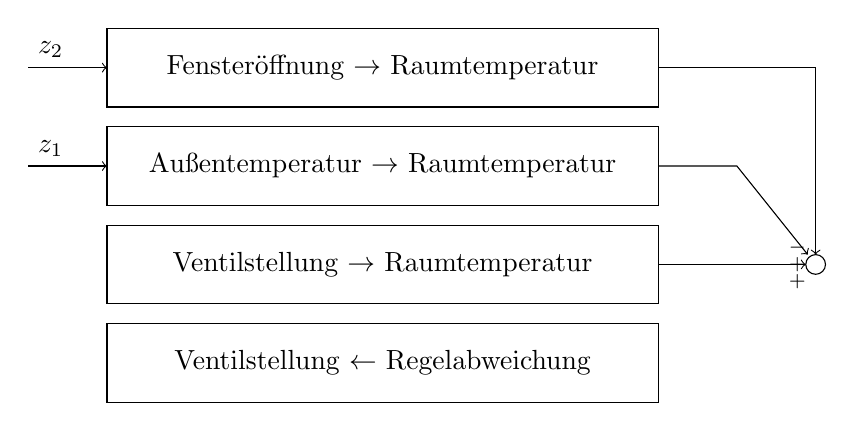
\begin{tikzpicture}
        \draw[->] (0,0) node[above right] {\(z_2\)} -- (1,0);
        \draw[->] (0,-1.25) node[above right] {\(z_1\)} -- (1,-1.25);
        \draw (1,-.5) rectangle (8,.5) node[pos=.5] {Fensteröffnung \(\to\) Raumtemperatur};
        \draw (1,-1.75) rectangle (8,-.75) node[pos=.5] {Außentemperatur \(\to\) Raumtemperatur};
        \draw (1,-3) rectangle (8,-2) node[pos=.5] {Ventilstellung \(\to\) Raumtemperatur};
        \draw (1,-4.25) rectangle (8,-3.25) node[pos=.5] {Ventilstellung \(\gets\) Regelabweichung};
        \draw (10,-2.5) circle (.125) node (a) {};
        \draw[->] (8,0) -- (10,0) -- (a) node[font=\scriptsize,above left] {\(-\)};
        \draw[->] (8,-1.25) -- (9,-1.25) -- (a) node[font=\scriptsize,left] {\(+\)};
        \draw[->] (8,-2.5) -- (a) node[font=\scriptsize,below left] {\(+\)};
    \end{tikzpicture}
	\caption{Schematische Darstellung der Raumtemperaturregelung}
	\label{fig:1-2}
\end{figure}

Neben der Regelung der Raumtemperatur entsprechend den Bildern \ref{fig:1-1} und \ref{fig:1-2} ist auch eine Steuerung der Raumtemperatur weit verbreitet (Bilder \ref{fig:1-3}, \ref{fig:1-4}).
Dabei wird z.B. die Außentemperatur \(Z_1\) gemessen und das Heizungsventil durch ein Steuergerät \(S\) dieser Temperatur entsprechend eingestellt.
Wie die schematische Darstellung in Bild \ref{fig:1-4} zeigt, liegt hier kein in sich geschlossener Wirkungsablauf vor.
Außerdem können größere Abweichungen der Temperatur \(X\) vom gewünschten Wert auftreten, wenn die nicht erfasste Störgröße \(Z_2\) (hier Öffnen von Fenstern usw.) entsprechende Werte annimmt oder wenn der im Steuergerät enthaltene funktionale Zusammenhang zwischen Außentemperatur und Ventilstellung den Eigenschaften von Heizung und Gebäude nicht genau entspricht.
